\chapter{Additional and related research involving evidence evaluation, biomedical knowledge graphs, and pharmaceutical discovery}


\vspace*{\fill}
Projects described in this chapter:


\noindent
\ref{section:carlsbad} CARLSBAD: Confederated, annotated research library of small-molecule bioactivity data

\noindent
\ref{section:opddr} OPDDR: Open phenotypic drug discovery resource

\noindent
\ref{section:tinx} TIN-X: Target importance and novelty explorer

\vspace*{\fill}


\newpage
\section{CARLSBAD: Confederated, annotated research library of small-molecule bioactivity data}
\label{section:carlsbad}

\textbf{Publication}: The CARLSBAD Database: A Confederated Database of Chemical Bioactivities, S.L. Mathias et al., Database, 2013\cite{Mathias2013-hj}.\\
\textbf{Web application}: \href{https://datascience.unm.edu/tomcat/carlsbad/carlsbadone}{CarlsbadOne}\\
\textbf{Source code}: \href{https://github.com/unmtransinfo/CARLSBAD}{GitHub:CARLSBAD}

\subsection{Introduction}

CARLSBAD is an integrated, harmonized, chemically intelligent bioactivity knowledge graph.

Several bioactivity databases offer information regarding the biological activity of small molecules on protein targets. However, resolving, reconciling and integrating such data is challenging due to heterogeneity and lack of data standards, for chemicals, for protein targets, and for bioactivity experiments and measures. To address this problem, we developed CARLSBAD as an integrated resource, built from high-quality subsets from several bioactivity databases, aggregated and presented in a uniform manner, annotated with common chemical patterns (CCPs), with a user-friendly web interface, suitable for the study of the relationships between small molecules and targets. CARLSBAD provides scientists with novel ways of exploring chemical biology space to facilitate knowledge mining for drug discovery. 

\subsection{Background}

As the number of chemicals and screening efforts multiply, the number of bioactivity databases offering information on biological activity of small molecules is increasing. They represent a rich source of information in our quest to map the chemical space of bioactive molecules to phenotypic and target space. We estimate that the space of publicly available bioactivity data indexes over at least 1.15 million unique chemicals, annotated onto \textgreater 15,000 targets\cite{Kim_Kjaerulff2013-hi}. The exact magnitude of this space could be derived only if one could uniformly process these data into a single database and harmonize chemicals, targets, bioassays and bioactivities. 

\subsection{Results}

To address these harmonization challenges, and to achieve consistency and coherence among disparate chemical—target bioactivity pairs, we developed CARLSBAD (Confederated Annotated Research Libraries of Small molecule BioActivity Data), integrating and harmonizing bioactivity data from the following sources: ChEMBL\cite{Gaulton2017-gp}, IUPHAR\cite{Harding2018-ut}, PDSP\cite{Roth2000-bh} (4), PubChem\cite{Kim2021-dv} and WOMBAT\cite{Olah2005-zd}. In addition, the KEGG database\cite{Ogata1999-he} diseases associated with targets were loaded to support disease queries.

The CARLSBAD workflow generates a single normalized, best-confidence activity value for each unique chemical–protein target pair. CARLSBAD contains 439,985 unique chemical structures, mapped onto 1,420 889 unique bioactivities. Of the 890,323 unique structure–target pairs curated in CARLSBAD, 13.95\% are aggregated from multiple structure–target values: 94,975 are aggregated from two bioactivities, 14,544 from three, 7930 from four and 2214 have five bioactivities, respectively.  CARLSBAD captures bioactivities and tags for 1435 unique chemical structures of active pharmaceutical ingredients (i.e. ‘drugs’). 

Two published cheminformatics methods have been implemented to perceive chemotypes, or common chemical patterns (CCPs): (1) HierS (hierarchical scaffolds) and (2) MCES (maximum common edge subgraph). CARLSBAD includes 277,140 HierS scaffolds and 54,135 MCES chemical patterns, respectively. These chemotypes provide a powerful tool for organizing, analyzing, discovering and visualizing bioactivity patterns and knowledge.

The focus on high-quality subsets of data from the five aforementioned databases was a major determinant for CARLSBAD, which aggregates chemical bioactivity information for drug discovery and repurposing activities from five different sources, shown earlier in the text. Only bioactivities that can be normalized to negative log molar values were processed for inclusion in the aggregated database. No single-point bioactivity values or phenotypic/cellular assay data were captured. In the current release, CARLSBAD includes only activity values associated with protein targets from human, mouse and rat. All activity data from the source databases that satisfy the aforementioned criteria are stored in the CARLSBAD database.

For the purpose of data mining, patent analytics and decision making, a single (highest confidence) activity value for any given bioactivity type, e.g. inhibition constant, Ki, or effective concentration at which 50\% of the response is obtained (EC50) is calculated, and returned for each unique chemical–protein target pair (‘CARLSBAD activity’). CARLSBAD activities correspond to unique four-tuples (chemical, protein, species, activity-type). For example, the cholesterol-lowering drug lovastatin has only one activity of type Ki on the human HMG CoA reductase protein (the rate-limiting enzyme in the metabolic pathway that produces cholesterol) stored in the CARLSBAD database. To generate these unique four-tuples, we defined confidence levels to establish a hierarchy for data sources during aggregation. When multiple activity values of the same type (e.g. Ki) with equal confidence levels were found, the mean value was indexed.

CARLSBAD CCPs are pre-calculated and stored for all chemical structures in the database, using the maximum common edge subgraph (MCES) and hierarchical scaffold (HierS) algorithms. MCES and HierS are complementary, as each method perceives structural chemotypes in a different manner. The cross-indexing of bioactivity, target and CCP data enables scientists to perform multiple tasks related to data mining, hypothesis generation and chemical biology space exploration. Classes of structural features that might be responsible for invoking certain biological responses can thus be examined within the CARLSBAD platform. Alternatively, biological targets could be categorized based on their preference toward particular CCPs.

\begin{figure}
    \centering
    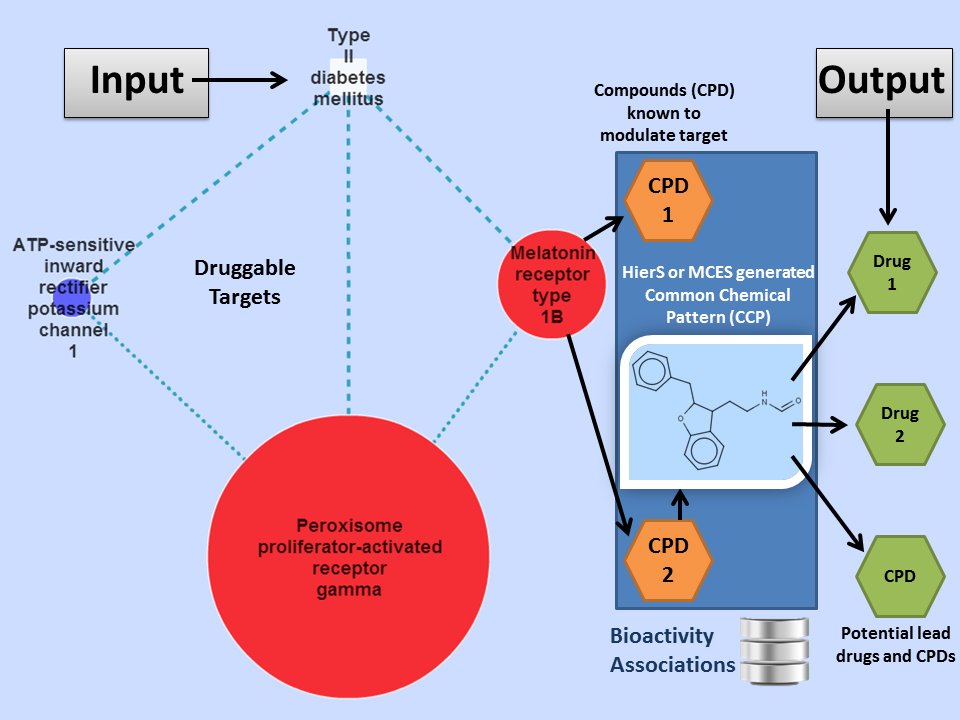
\includegraphics[width=\textwidth]{figures/carlsbad/CB1_Screenshots.png}
    \caption{CARLSBAD schematic}
    \label{fig:cb_schematic}
\end{figure}

The CARLSBAD database is implemented as a PostgreSQL relational database with entities such as substance, compound, activity, target and so forth, and the various relationships between them (figure \ref{fig:cb_erd}). The CHORD chemical cartridge from \href{https://www.gnova.com/}{gNova Scientific Software} is used to provide fast chemical functionalities such as SMILES canonicalization\cite{Weininger1989-kh}, chemical fingerprints and structure searching. CHORD is based on the OEChem toolkit, available from \href{https://www.eyesopen.com/}{OpenEye Scientific Software}.


Separate extract, transform and load (ETL) pipelines were built for each of the data sources. The sections later in the text detail the specific source of data used and the extraction criteria applied for each.

\textbf{ChEMBL}. A MySQL dump of ChEMBL v13, 2012–02–21 was downloaded from the website. ChEMBL data passing the following filters were loaded into CARLSBAD: only activities from publications were loaded; activities associated with pharmacokinetic, cellular and in vivo assays, and any other activities not associated with a protein target were not imported; activities not associated with human, rat and mouse targets were skipped; and activities without values or units that could be converted to -log(molar) were also skipped. Activities of the following type were loaded: EC50, IC50, pEC50, pIC50, Log EC50, Log IC50, Ki, Kb, Kd, pKi, pKb, pKd, Log Ki, Log Kb, LogKd, ED50, IC80, IC90, A2, D2, pA2, pD2 and Km. Also, activities with units expressed in molarity, as well as activities with an associated structure were loaded. Additionally, activity values were converted to molar wherever necessary and converted to negative log where appropriate.

\textbf{IUPHAR}. Data were programmatically extracted from the \href{http://www.iuphar-db.org/}{IUPHAR website} (February 2011). Only activities with the following classes were loaded: agonists, antagonists, pore blockers, activators, allosteric regulators, gating inhibitors and channel blockers. In addition, midpoints or medians were used for affinities expressed as ranges. Activities not associated with human, rat and mouse targets as well as activities with unknown affinities or units were excluded.

\textbf{PDSP}. The text file (kidb110121.txt) was downloaded from the \href{http://pdsp.med.unc.edu/indexR.html}{PDSP website}. UniProt IDs were added to this file by the group of Stephan Sch\"{u}rer, University of Miami. This file was used as the source from which data were extracted and used to populate the CARLSBAD database. Activities associated with structures not parseable by gNOVA, and activities with qualified values (i.e. \textgreater x) were skipped.

\textbf{PubChem}. Only confirmatory assays with human, rat or mouse protein targets from the Molecular Libraries Program (query filters: ‘Molecular Libraries Probe Production Centers Network[SourceCategory]’, confirmatory[Filter] and pcassay\_protein\_target[Filter]) were considered for CARLSBAD. Only activities with values, molarity units, associated compounds, and the following result types were loaded: various versions of EC50, AC50, IC50, Ki and Potency. Additionally, activity values were converted to molarity if necessary, and activity values were converted to negative Log10 if necessary.

\textbf{WOMBAT}. Version 2011.2 (SDF and activities.tab files) was used as the source from which data were extracted and used to populate the CARLSBAD database. Only activities of the following types were loaded: EC50, ED50, IC50, IC80, IC90, Ki, Kb, Kd, Km, A2 and D2. In addition, the following data were skipped: activities not associated with a known target; activities not associated with human, rat and mouse targets; activities associated with targets without an associated UniProt identifier; activities from primary screening; activities labeled ‘inactive’; and activities with descriptive values (e.g. ‘active’).

\textbf{KEGG}. From 1301 total KEGG disease terms, 308 associated by KEGG with CARLSBAD protein targets were loaded for availability as disease queries.

When pairing structures with targets and bioactivities in a similar effort, Tikkainen and Franke observed that only 3.6\% (i.e. 410 of 11,278) of the scientific articles with activity indexed in more than one database matched each other. Indeed, data discrepancies are ubiquitous as far as data curation is concerned\cite{Tiikkainen2012-cw}. The processing log for CARLSBAD is summarized in table \ref{tab:cb_01}: of 975,117 unique structure–target pairs in the database, 84,794 were found unique to WOMBAT and, therefore, have not been processed into CARLSBAD. For the remaining 890,323 structure–target pairs, 124,231 (13.95\%) were aggregated from multiple structure–target values: 94,975 from two bioactivities, 14,544 from three, 7930 from four and 2214 from five bioactivities, respectively. The highest number of consolidated bioactivities is 109, with the second highest number being 106. As data aggregation is the intended purpose for CARLSBAD, we focused on eliminating extremes in the bioactivity spectrum, and aggregating values towards a mean value. Hierarchical processing (i.e. confidence levels) was used in $\sim$25\% of the cases (192,736 + 38,670 substance–target pairs) when generating the CARLSBAD activity.

\begin{table}
\caption{CARLSBAD database consolidation process summary}
\label{tab:cb_01}
\centering
\begin{tabular}{l|c}
\hline
\textbf{Bioactivities} & \textbf{Substance–target pairs} \\
\hline
Initial aggregated data & 975,117\\
Valid processed pairs & 975,110\\
WOMBAT only & 84,794\\
Only one activity on record & 658,917\\
Only one activity type (each entered) & 192,736\\ 
Multiple activity types processed & 38,670\\
total activities loaded & 932,881\\
\hline
\end{tabular}
\end{table}


\textbf{Web interface "CarlsbadOne"}. A web interface to the CARLSBAD database was developed:  \href{https://datascience.unm.edu/tomcat/carlsbad/carlsbadone}{CarlsbadOne}. The web application is written Java and deployed as a Java Web Application via Apache Tomcat, and uses JChem from ChemAxon for cheminformatics. Users can query by target, drug, or disease. Figures \ref{fig:cb_cbone_01} and \ref{fig:cb_cbone_02} illustrate a query for drug "Marinol". Figures \ref{fig:cb_cbone_04} and \ref{fig:cb_cbone_05} illustrate a query for disease "Type 1 Diabetes".

\begin{figure}
\centering
\begin{subfigure}{0.8\textwidth}
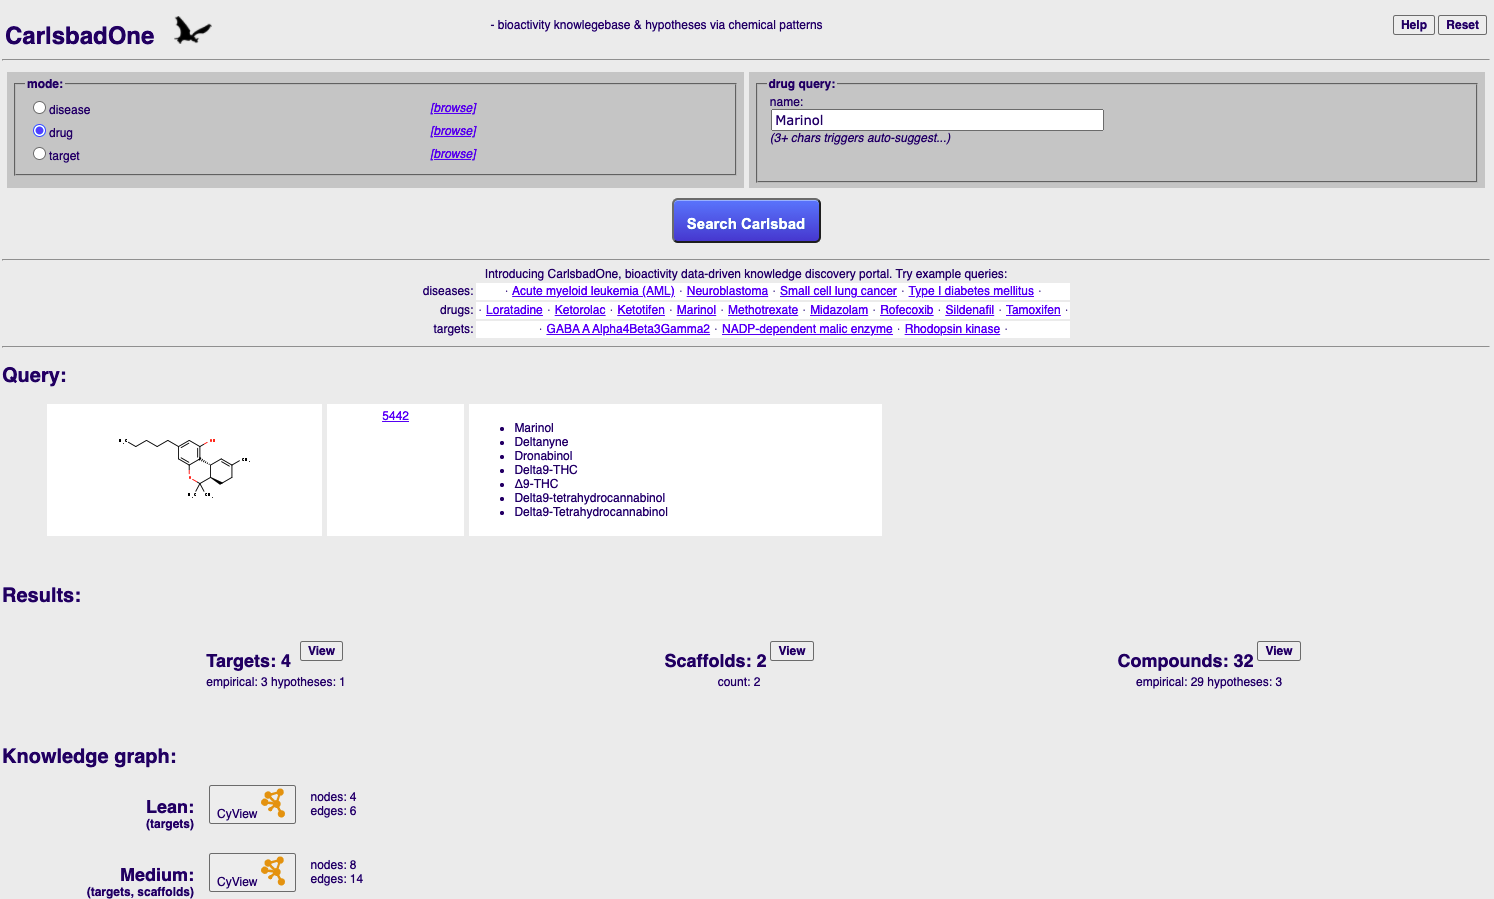
\includegraphics[width=0.95\linewidth]{figures/carlsbad/CARLSBAD_CBOne_Marinol_01.png} 
\caption{CarlsbadOne, drug query Marinol}
\label{fig:cb_cbone_01}
\end{subfigure}
\begin{subfigure}{0.8\textwidth}
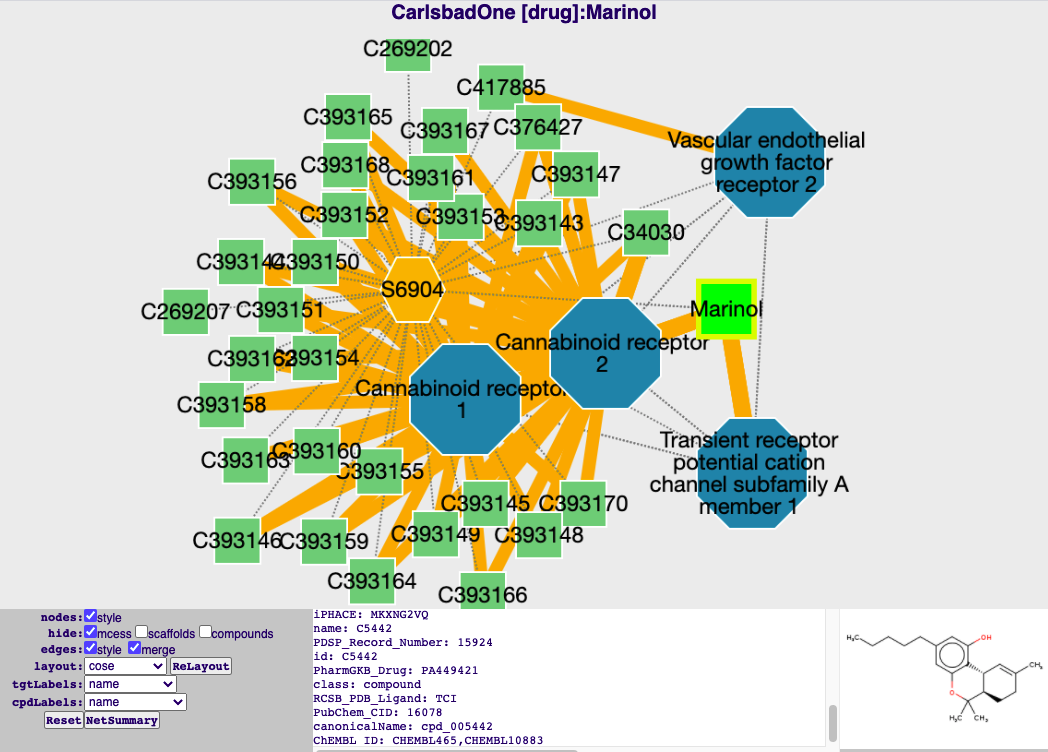
\includegraphics[width=0.95\linewidth]{figures/carlsbad/CARLSBAD_CBOne_Marinol_02.png}
\caption{CarlsbadOne, drug query Marinol, results subgraph}
\label{fig:cb_cbone_02}
\end{subfigure}
\caption{CarlsbadOne, drug query Marinol, results subgraph}
\label{fig:cb_cbone_03}
\end{figure}


\begin{figure}
\centering
\begin{subfigure}{0.8\textwidth}
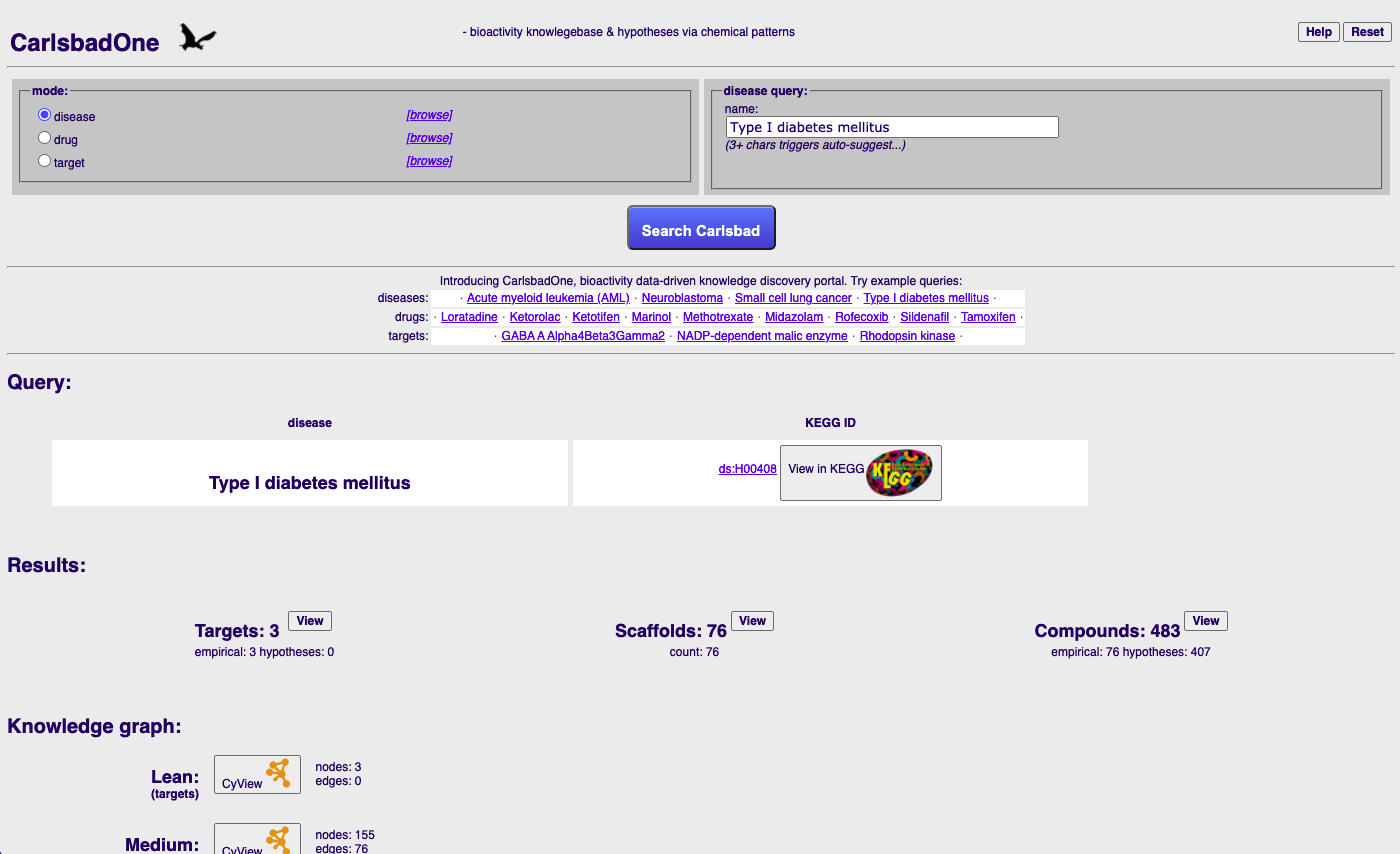
\includegraphics[width=0.95\linewidth]{figures/carlsbad/CARLSBAD_CBOne_T1DM_01.png} 
\caption{CarlsbadOne, disease query Type 1 Diabetes}
\label{fig:cb_cbone_04}
\end{subfigure}
\begin{subfigure}{0.8\textwidth}
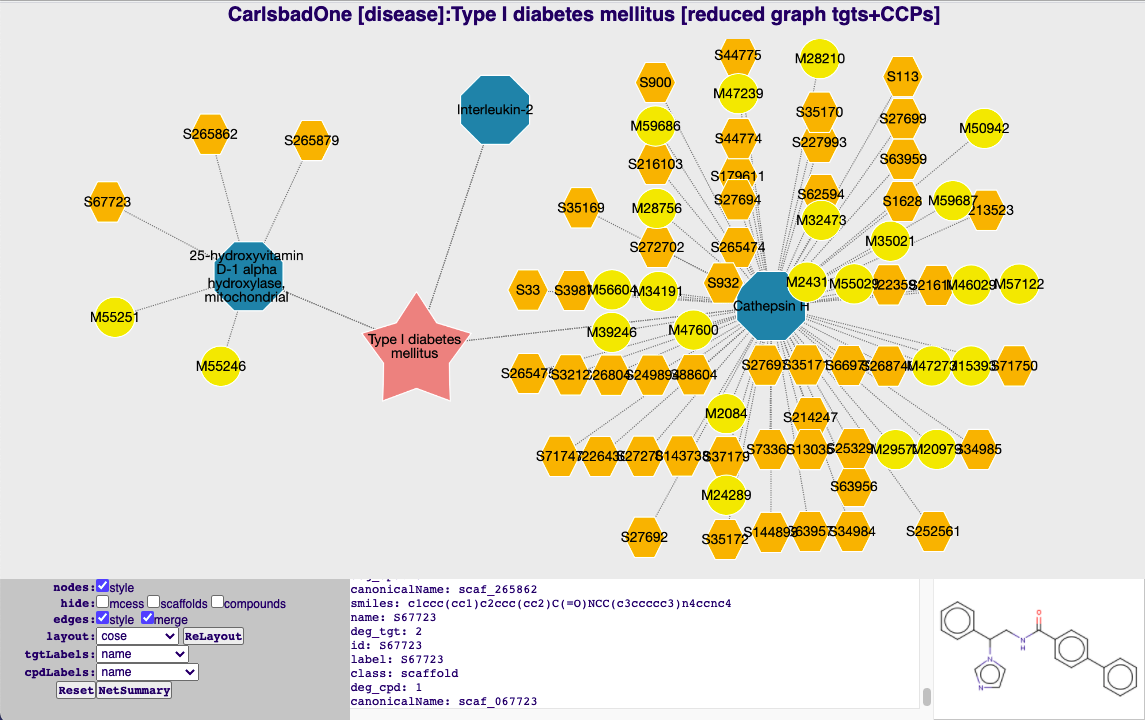
\includegraphics[width=0.95\linewidth]{figures/carlsbad/CARLSBAD_CBOne_T1DM_02.png}
\caption{CarlsbadOne, disease query Type 1 Diabetes, results subgraph}
\label{fig:cb_cbone_05}
\end{subfigure}
\caption{CarlsbadOne, disease query Type 1 Diabetes, results subgraph}
\label{fig:cb_cbone_06}
\end{figure}


\subsection{Methods}

\subsubsection{Target curation}

Source databases vary in their use of identifiers for gene and protein targets, creating challenges to accurate mapping and resolution. Consequently, care was taken to accurately map source targets to UniProt accession IDs, and annotate with data from UniProt\cite{UniProt_Consortium2018-kq}: name, description, sequence, other identifiers (NCBI gi, RefSeq, Gene, UniGene and PDB), and also classifiers (InterPro, Pfam and PROSITE domains; GO terms; and UniProt family).

\subsubsection{Disease curation}

The Kyoto Encyclopedia of Genes and Genomes (KEGG) is pathway-centric but includes molecules, cells, organisms, diseases and drugs, as well as relationships among them\cite{Kanehisa2008-zv}. For CARLSBAD, only the diseases associated with protein coding genes were loaded into the CARLSBAD database.

\subsubsection{Chemical curation}

In the CARLSBAD database, chemical substances are distinguished from compounds in accordance with PubChem terminology. In this paradigm, compounds represent the abstract structure of any of the components of the substance. Chemical structures are stored as canonical SMILES using CHORD (gNova/OpenEye).  In addition, 26 chemical descriptors are calculated and stored for each unique compound. These descriptors (e.g. molecular weight, number of rings and so forth) are provided for convenience to users interested in specific subsets of chemical space. Finally, common chemical patterns (CCPs) HierS and MCES are calculated and associated with the corresponding chemical structures.

\subsubsection{HierS}

HierS, the hierarchical scaffold grouping algorithm\cite{Wilkens2005-ja} (9), is based on the molecular framework concept described by Bemis and Murcko\cite{Bemis1996-jg}. The ‘scaffold’ concept is central in medicinal chemistry and provides a chemically intuitive manner to visualize chemical classes, as ring-based linkages are central structural features in most (\textgreater 90\%) drug molecules. The algorithm relates any two compounds by their common shared scaffolds. Scaffolds generally have two advantages over MCS: (i) computational speed and (ii) chemical interpretability. To our knowledge, there is no currently available implementation of HierS in any commercial or open-source package. We have implemented these tools in an open-source Java library \href{https://github.com/unmtransinfo/unm_biocomp_hscaf}{HScaf}\cite{Yang2012-qd} built on the JChem toolkit from ChemAxon.

\subsubsection{MCES}

MCES. The maximum common edge subgraph (MCES) concept\cite{Raymond2002-ep} can be used to compute similarity between two molecular graphs and has been widely used in many applications\cite{Stahl2005-bl,Sheridan2006-nx,Gardiner2007-ur,Bocker2008-uh,Hariharan2011-qx,Bostrom2012-fb}. However, MCES is computationally expensive (NP complete) and infeasible for large datasets such as CARLSBAD. Thus, additional heuristics are needed to reduce computational time. As HierS is efficient and fast, HierS scaffolds were used to group compounds based on common scaffolds. With this heuristic, pairwise MCES was computed between compounds sharing the same scaffolds. The resulting MCESes thereby define groupings of compounds with shared maximum common substructures.

\subsection{Discussion}

The availability of massive amount of molecular bioactivity data creates rich new opportunities, yet for typical scientists involved in biomedical discovery research, the difficulty of processing and analyzing that data can often be a barrier. With the occasional, less experienced end-user in mind, we have developed a small molecule bioactivity database that facilitates navigation in the small molecule/bioactivity space. The unique features and underlying data structure of the CARLSBAD database are designed to support polypharmacology-driven drug discovery scenarios, such as drug repurposing, side effect/off-target prediction and lead identification workflows.

The net result of chemical, bioactivity and target aggregation, curation and harmonization is summarized in table \ref{tab:cb_02}: the number of substances, i.e. chemicals tested for bioactivity, is smaller than the one obtained by summing the five databases by 17.27\%. A similar trend is observed when examining bioactivities (34.35\% reduction) and CCPs (23.1\% reduction using HierS and 25\% using MCES). The aforementioned values are the result of machine-based harmonization and consolidation of multiple data objects in chemical, bioactivity and CCP space. An independent study by Tiikkainen and Franke\cite{Tiikkainen2013-md,UniProt_Consortium2018-kq}, comparing ChEMBL (release 14) and WOMBAT 2012.01, showed \textgreater 394,000 unique bioactivities in WOMBAT, compared with nearly 3.3 million bioactivities in ChEMBL; and 2755 unique targets in ChEMBL, compared with 1486 unique targets in WOMBAT. The harmonization trends suggest that a consolidated database is preferable to a federated collection, at least in this case, when seeking to evaluate global bioactivity trends. This solution was, for example, implemented in the ‘Merz Virtual Bioactivity Database’, which integrates ChEMBL and WOMBAT, among other data sources.

\begin{table}
\caption{Overview of the numbers of substances, activities and CCP data in the original databases, as well as the consolidated CARLSBAD database}
\label{tab:cb_02}
\centering
\begin{tabular}{p{0.25\linewidth}p{0.15\linewidth}p{0.15\linewidth}p{0.15\linewidth}p{0.30\linewidth}}
\hline
\textbf{Source (Version)} & \textbf{Release date} & \textbf{Structures} & \textbf{Activities} & \textbf{CCPs} \\
\hline
ChEMBL (13) & 2012–02–21 & 267,744 & 798,755 & \makecell[l]{182,496 scaf \\ 32,794 mces} \\
IUPHAR & 2011 & 2297 & 6049 & \makecell[l]{2704 scaf \\ 652 mces} \\
PDSP (kidb110121) & & 3499 & 22,202 & \makecell[l]{3422 scaf \\ 823 mces} \\
PubChem (MLP) & 2011–11–04 & 133,435 & 320,311 & \makecell[l]{83,570 scaf \\ 20,867 mces} \\
WOMBAT & 2011.2 & 124,873  & 273,572 & \makecell[l]{88,135 scaf \\ 17,086 mces} \\
\hline
Total & & 531,848 & 1,420,889 & \makecell[l]{360,327 scaf \\ 72,222 mces} \\
\hline
CARLSBAD & 2012.1 & 439,985 & 932,881 & \makecell[l]{277,140 scaf \\ 54,135 mces} \\
\hline
\end{tabular}
\end{table}

Comparing the databases, it is apparent that ChEMBL is the most populated in terms of substances, bioactivities and CCPs, followed by WOMBAT and PubChem/MLP. This is to be expected, given their chemogenomic purpose. Two of the databases dedicated to pharmacology, IUPHAR and PDSP, are significantly smaller. An in-depth comparison with respect to targets, bioactivities and chemistry coverage for some of these databases has been performed\cite{Tiikkainen2012-cw}. Each of these databases provided relevant contributions in terms of CARLSBAD aggregation.

Chemical errors were addressed with focus on the high-value, high-confidence IUPHAR and PDSP subsets. We found only one PDSP structure that was not parsable by gNova/OEChem; it was manually corrected. For IUPHAR, we extensively curated \textgreater 2700 small molecules and peptides from IUPHAR’s ‘Ligand List’ (http://www.iuphar-db.org/DATABASE/LigandListForward: retrieved 2011-02-04). This curation involved reading the original ligand references to resolve ligand names, 2D structures and biological activities, including \textgreater700 peptides for which structural information was not then available in IUPHAR-DB\cite{Harding2018-ut}. 

When aggregating data in CARLSBAD, we did not explicitly address biology or bioactivity errors. By cross-referencing PubMed IDs for literature-based data (i.e. PDSP, IUPHAR-DB, ChEMBL and WOMBAT), we found that identical articles are covered by these resources, yet data are not always identical. Indeed, up to 3\% errors in target protein identity, up to 2.7\% errors in bioactivity values, and up to 7\% errors in chemical structure depiction were found in comparing three data sources. In CARLSBAD, these tuples were harmonized by providing median values wherever possible, and by representing ‘higher curation’ values where possible, when multiple conflicting values were found. For example, bioactivity results from IUPHAR-DB were given the highest priority, as they summarize the significant curation effort made by members of the IUPHAR Nomenclature Committee. Overall, this situation occurred in \textless 10\% of the database. With respect to data generated by the NIH Molecular Libraries Initiative\cite{Austin2004-qc}, only data from PubChem was uploaded into CARLSBAD, as stated earlier in the text. Thus, any bioactivity value ‘feedback loop’, i.e. propagation of errors from one database to another, was avoided by importing non-overlapping sets of data.

Chemical space overlap between structures in the CARLSBAD database and drugs approved for human use was determined using structure identity comparison with an in-house curated database of drug structures approved worldwide, which includes discontinued drugs as well\cite{Oprea2010-kd,Manallack2013-qm}. A total of 1435 unique chemical structures for active pharmaceutical ingredients (i.e. ‘drugs’) were identified in CARLSBAD of $\sim$4000 small organic molecules. These chemical structures were flagged accordingly for user convenience and can be used to explore biological activity space of known drugs.

\subsection{Conclusion}

CARLSBAD is a database focused on high-quality subsets aggregated from several bioactivity databases, which are integrated in a uniform interface and manner, suitable for chemical biology and drug discovery studies, as well as large scale, ‘big data’ informatics and knowledge mining. In contrast to the original data collections, CARLSBAD provides a single normalized activity value of a given type for each unique chemical–protein target pair. Aggregation accounted for $\sim$25\% of the \textgreater 975,000 structure–target pairs processed, up to and including 109 bioactivities for a single chemical. We implemented two types of chemotype perception for common chemical patterns, HierS and MCES. CARLSBAD contains 439,985 unique chemical structures, mapped onto 1,420,889 unique bioactivities and annotated with 277,140 HierS scaffolds and 54,135 MCES patterns, respectively. It also contains bioactivities and tags for 1435 unique active pharmaceutical ingredients.

\subsection{Researcher contributions}

CARLSBAD was very much a collaborative team effort, involving many meetings and interactions among members, but also with designated roles and tasks. JY was a major contributor (\href{http://purl.org/spar/scoro/major-effort}{scoro:major-effort}) fully engaged in the team effort, and also responsible for research and development tasks, specifically:

\begin{itemize}[topsep=0pt,itemsep=0pt,partopsep=0pt,parsep=0pt]
    \item Scientific software development of web applications SNAKE and CarlsbadOne. These Java web applications were developed iteratively, with ongoing feedback from scientific users, to address pharmaceutical research use cases. The addition of KEGG diseases and disease queries was a notable result of scientific user feedback\\ (\href{http://purl.org/spar/scoro/IntellectualContribution}{scoro:IntellectualContribution}, \href{http://purl.org/spar/scoro/OrganizationalContribution}{scoro:OrganizationalContribution}).
    \item Support, documentation, outreach (conference talk, etc.) and publication\\
    (\href{http://purl.org/spar/scoro/AuthorshipContribution}{scoro:AuthorshipContribution}). 
\end{itemize}

%\rule[0.5ex]{\linewidth}{2pt}
\newpage

\section{OPDDR: Open phenotypic drug discovery resource}
\label{section:opddr}

\textbf{Publication}: Novel Phenotypic Outcomes Identified for a Public Collection of Approved Drugs from a Publicly Accessible Panel of Assays, J. Lee, et al, PLoS ONE, 2015\cite{Lee2015-vg}.\\
\textbf{Source code}: \href{https://github.com/IUIDSL/OPDDR}{GitHub:OPDDR}\\
\textbf{PubChem}: \href{https://pubchem.ncbi.nlm.nih.gov/bioassay/1117321}{BioAssay:1117321}\\
\textbf{Poster}: \href{https://doi.org/10.5281/zenodo.4844529}{https://doi.org/10.5281/zenodo.4844529}

\subsection{Introduction}

Phenotypic assays have a proven track record for generating leads that become first-in-class therapies. Whole cell assays that inform on a phenotype or mechanism also possess great potential in drug repositioning studies by illuminating new activities for the existing pharmacopeia. The National Center for Advancing Translational Sciences (NCATS) pharmaceutical collection (NPC) is the largest reported collection of approved small molecule therapeutics that is available for screening in a high-throughput setting. Via a wide-ranging collaborative effort, this library was analyzed in the Open Innovation Drug Discovery (OIDD) phenotypic assay modules publicly offered by Lilly. 

This project involved the characterization of 2460 clinical phase/approved drugs in five Lilly OIDD phenotypic assays. The work was part of an ongoing collaboration involving Lilly, NIH-NCATS, and Data2Discovery.  The focus of this description of OPDDR is the informatics: transforming and integrating data to enhance semantic value, development of a knowledge graph (KG) -- a.k.a. knowledge network (KN), a publicly shared Open Phenotypic Drug Discovery Resource (OPDDR, aka PD2) which can be used to identify relationships between National Pharmaceutical Collection (NPC) compounds, phenotypic assays, ontological classes of assays, and associated public data on related molecular targets. The results of these tests are publically available online at \href{https://www.ncats.nih.gov/expertise/preclinical/pd2}{NCATS} and via PubChem (\href{https://pubchem.ncbi.nlm.nih.gov/bioassay/1117321}{BioAssay:1117321}).

\subsection{Results}

The significantly revised (June 2015) PubChem RDF data model was integrated, informed via engagement with PubChem team (Bolton et al.). BioAssay Ontology (BAO) integration informed by discussions with BAO team (Sch\"urer et al.), and with AstraZeneca (Enqvist) regarding their assay annotation template. OpenPHACTS (OP) integration informed by discussions with the OP team, which entailed major revisions in the KN, and also revisions in the OP data model and API, to handle phenotypic assays. Figure \ref{fig:opddr_01} illustrates the OPDDR RDF schema, or data model, grouped by data source.

\begin{figure}
    \centering
    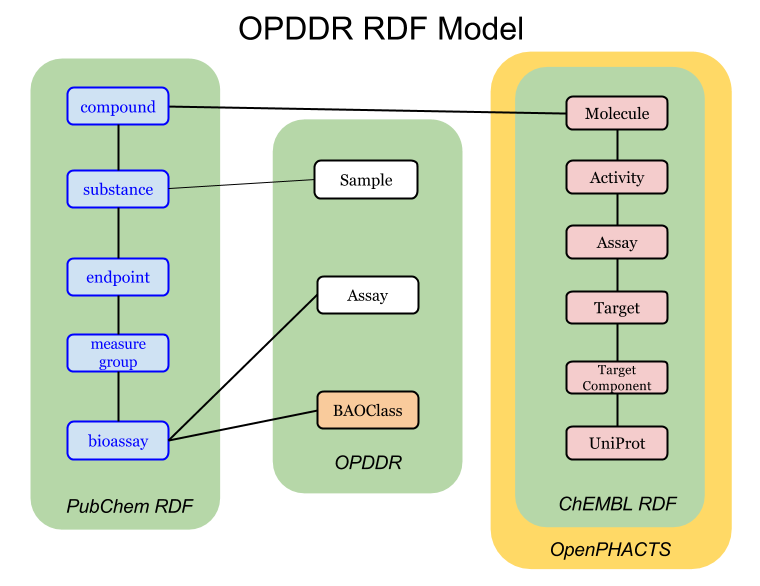
\includegraphics[width=\linewidth]{figures/opddr/OPDDR_schema.png}
    \caption{OPDDR RDF schema, simplified, showing source relationships.}
    \label{fig:opddr_01}
\end{figure}

\subsubsection{Knowledge graph description}

The initial version of the KG is intended to provide a clear and easily comprehensible first step of describing the OPDDR compounds and assays in accordance with standardized community ontologies and namespaces, and relating these to protein targets from ChEMBL.  Biological networks can be extremely complex, and many further entity classes can be integrated in future (e.g. pathways), and will be facilitated by this initial KG.

\subsection{Methods}

\subsubsection{Ontologies Used}

The KG uses the ontologies listed in table \ref{tab:opddr_01}.

\begin{table}
\caption{Ontologies}
\label{tab:opddr_01}
\centering
\begin{tabular}{p{0.25\linewidth}p{0.75\linewidth}}
\hline
\textbf{PubChem RDF} & \href{http://rdf.ncbi.nlm.nih.gov/pubchem/}{PubChem RDF Schema}. Primary reference for this project.  Mainly because assays and substances have been deposited into PubChem.\\
\hline
\textbf{BAO} & \href{http://www.bioassayontology.org/bao\#}{Bioassay Ontology}.  Initially using a minimal set based on annotation template provided by AstraZeneca.  Only bao\_vocabulary\_assay.owl is required currently.\\
\hline
\textbf{ChEMBL RDF} & \href{http://rdf.ebi.ac.uk/terms/chembl\#}{ChEMBL RDF Schema and ChEMBL Core Ontology (CCO)}. 
\\
\hline
\textbf{BFO} &  \href{http://purl.obolibrary.org/obo/}{Basic Formal Ontology}\\
\hline
\textbf{SIO} & \href{http://semanticscience.org/resource/}{Semanticscience Integrated Ontology}\\
\hline
\end{tabular}
\end{table}

\subsubsection{Entities}

The KG includes the entities listed in table \ref{tab:opddr_02}.

\begin{table}
\caption{OPDDR entities}
\label{tab:opddr_02}
\centering
\begin{tabular}{p{0.7\linewidth}p{0.3\linewidth}}
\hline
\makecell[c]{\textbf{namespace}} & \textbf{example} \\
\hline
\makecell[r]{http://rdf.ncbi.nlm.nih.gov/pubchem/substance/} & SID124893119 \\
\makecell[r]{http://rdf.ncbi.nlm.nih.gov/pubchem/compound/} & CID1131 \\
\makecell[r]{http://rdf.ncbi.nlm.nih.gov/pubchem/bioassay/} & AID1117354 \\
\makecell[r]{http://rdf.ncbi.nlm.nih.gov/pubchem/measuregroup/} & AID1117354 \\
\makecell[r]{http://rdf.ncbi.nlm.nih.gov/pubchem/endpoint/} & SID124893119\_AID1117354 \\
\makecell[r]{http://rdf.ncbi.nlm.nih.gov/pubchem/protein/} & GI124375976 \\
\makecell[r]{http://rdf.ebi.ac.uk/resource/chembl/target/} & CHEMBL3038470 \\
\makecell[r]{http://rdf.ebi.ac.uk/resource/chembl/targetcomponent/} & CHEMBL\_TC\_1927 \\
\makecell[r]{http://rdf.ebi.ac.uk/terms/chembl\#\textit{UniprotRef}} & P53350 \\
\makecell[r]{http://rdf.ebi.ac.uk/resource/chembl/assay/} & CHEMBL987214 \\
\makecell[r]{http://rdf.ebi.ac.uk/resource/chembl/activity/} & CHEMBL\_ACT\_2470294 \\
\makecell[r]{http://rdf.ebi.ac.uk/resource/chembl/molecule/} & CHEMBL44884 \\
\hline
\end{tabular}
\end{table}

Note that PubChem compounds are required in addition to substances.  Compounds refer to canonically defined and identifiable chemical entities which can be linked across databases; Substances refer to specific samples of compounds as provided by a supplier.  We thus include both, to be as comprehensive and specific as possible.   Note also that PubChem measuregroups are defined for each assay, for example, the measuregroup URI for AID12345 is http://rdf.ncbi.nlm.nih.gov/pubchem/measuregroup/AID12345.  PubChem endpoints represent activity outcomes.  ChEMBL RDF represents bioactivities somewhat differently than PubChem, but we can rigorously link these data via chemical structure and CIDs.

\begin{table}
\caption{OPDDR KG Statistics}
\label{tab:opddr_03}
\centering
\begin{tabular}{p{0.3\linewidth}p{0.2\linewidth}p{0.5\linewidth}}
\hline
\textbf{type} & \textbf{count} & \textbf{notes} \\
\hline
substance & 2511 & PubChem SIDs \\
compound & 2511 & PubChem CIDs \\
assay & 35 & PubChem AIDs.  Summary AID is 36th. \\
measuregroup & 35 & PubChem AIDs.  Default for assay. \\
endpoint & 2511*35 & PubChem SID-AID pairs. \\
targets & 4977 & ChEMBL IDs.  All single-component. \\
protein & 4977 & A.k.a. target component.  With UniprotRefs. \\
protein activity & 584,157 & From ChEMBL, but includes PubChem data. \\
PD2 activity & 5320 & All “ACTIVE” outcomes from results. \\
assay classifications & 155 & Manually curated PD2 to BAO associations.  Exported from worksheet. \\
\hline
\end{tabular}
\end{table}

\begin{table}
\caption{OPDDR asserted triplets, patterns and examples.}
\label{tab:opddr_04}
\centering
\begin{tabular}{p{0.25\linewidth}p{0.75\linewidth}}
\hline
\textbf{description} & \textbf{examples} \\
\hline
assay to BAO class & \makecell[l]{\texttt{bioassay:AID1117354 rdf:type bao:BAO\_0000015}} \\ 
assay title & \makecell[l]{\texttt{bioassay:AID1117354 dcterms:title} \\ \texttt{"human JAK2 kinase inhibition-screen"@en}} \\
assay to measuregroup & \makecell[l]{\texttt{bioassay:AID1117354} \\ \texttt{bao:BAO\_0000209 measuregroup:AID1117354}} \\
substance to NCGC ID & \makecell[l]{\texttt{substance:SID144206486} \\ \texttt{skos:exactMatch ncats\_sample:NCGC00182710-02 .}} \\
substance to measure group & \makecell[l]{\texttt{substance:SID124882766 obo:BFO\_0000056} \\ \texttt{measureg:AID1117326}} \\
endpoint outcome (activity) & \makecell[l]{\texttt{endpoint:SID170466632\_AID743241} \\ \texttt{vocabulary:PubChemAssayOutcome vocabulary:inactive}} \\
endpoint class & \makecell[l]{\texttt{endpoint:SID103164874\_AID443491 rdf:type} \\ \texttt{bao:BAO\_0000190}} \\
substance to compound association & \makecell[l]{\texttt{substance:SID124893119} \\ \texttt{sio:CHEMINF\_000477 compound:CID1131}} \\
assay to OIDD ID & \makecell[l]{\texttt{bioassay:AID1117350 skos:exactMatch} \\ \texttt{oidd\_assay:17}} \\
ChEMBL target to UniProt & \makecell[l]{\texttt{chembl\_target:CHEMBL5464} \\ \texttt{cco:targetXref uniprot:Q13546}} \\
ChEMBL target to assay & \makecell[l]{\texttt{chembl\_target:CHEMBL5464} \\ \texttt{cco:hasAssay assay:CHEMBL3110727}} \\
ChEMBL target to target component & \makecell[l]{\texttt{chembl\_target:CHEMBL1867} \\ \texttt{cco:hasTargetComponent} \\ \texttt{chembl\_targetcmpt:CHEMBL\_TC\_180}} \\
ChEMBL target component to Uniprot & \makecell[l]{\texttt{chembl\_targetcmpt:CHEMBL\_TC\_180} \\ \texttt{cco:targetCmptXref uniprot:P08913}} \\
ChEMBL assay to activity & \makecell[l]{\texttt{assay:CHEMBL3110727 cco:hasActivity} \\ \texttt{activity:CHEMBL\_ACT\_13890030}} \\
ChEMBL molecule to activity & \makecell[l]{\texttt{chembl\_molecule:CHEMBL313842} \\ \texttt{cco:hasActivity activity:CHEMBL\_ACT\_14447741}} \\
PubChem substance to ChEMBL molecule & \makecell[l]{\texttt{substance:SID225144242} \\ \texttt{skos:exactMatch molecule:CHEMBL1474122}}  \\
\hline
\end{tabular}
\end{table}

\subsubsection{Files}

The files comprising OPDDR are listed in table \ref{tab:opddr_05}.  Files are grouped below by source, each file from one source only.

\begin{singlespace}
\begin{longtable}{p{0.5\linewidth}p{0.5\linewidth}}
\caption{OPDDR files.}
\label{tab:opddr_05}\\
\hline
\makecell{\textbf{filename} \\ \textbf{source: description}} & \makecell[c]{\textbf{example}} \\
\hline
\makecell[l]{npcpd2\_assay.ttl \\ OPDDR: Assay links to OIDD namespace} & \makecell[l]{bioassay:AID1117326\\ skos:exactMatch oidd\_assay:4} \\
\hline
\makecell[l]{npcpd2\_bao.ttl \\ OPDDR: Manually curated BAO\\ classifications.} & \makecell[l]{bioassay:AID1117352\\ rdf:type bao:BAO\_0000219} \\
\hline
\makecell[l]{npcpd2\_substance.ttl \\ OPDDR: Substance links to NCATS\\ namespace.} & \makecell[l]{substance:SID170465644\\ skos:exactMatch \\ ncats\_sample:NCGC00160518-03} \\
\hline
\makecell[l]{bao\_vocabulary\_assay.owl \\ BAO: BAO module with bioassay\\ class hierarchy.} &  \\
\hline
\makecell[l]{pubchem\_vocabulary.owl \\ PubChem: module with bioactivity\\ terms etc.} & \\
\hline
\makecell[l]{pubchem\_pd2\_assay.ttl \\ PubChem: RDF, includes titles, \\ measuregroups. } & \makecell[l]{bioassay:AID1117356 \\ bao:BAO\_0000209 \\ measuregroup:AID1117356\\ bioassay:AID1117351 \\ dcterms:title \\ "Increased HeLa cells \\ with 4N DNA content-IC50"@en}  \\
\hline
\makecell[l]{pubchem\_pd2\_substance.ttl \\ PubChem: RDF, includes CIDs,\\ measuregroups. } & \makecell[l]{substance:SID124882766\\ obo:BFO\_0000056 measuregroup:AID1117326 .\\ endpoint:SID124882766\_AID1117342\\ obo:IAO\_0000136\\ substance:SID124882766 .} \\
\hline
\makecell[l]{pubchem\_pd2\_endpoint.ttl \\ PubChem: RDF, includes endpoints,\\ activity results.} & \makecell[l]{endpoint:SID170464708\_AID1117354\\ obo:IAO\_0000136 substance:SID170464708 ;\\ vocabulary:PubChemAssayOutcome\\ vocabulary:inactive .\\ measuregroup:AID1117354\\ obo:OBI\_0000299\\ endpoint:SID170464708\_AID1117354 .} \\
\hline
\makecell[l]{chembl\_cco.ttl \\ ChEMBL: Core Ontology} & \\
\hline
\makecell[l]{chembl\_target.ttl \\ ChEMBL: protein targets.} & \makecell[l]{chembl\_target:CHEMBL2366239\\ a cco:SingleProtein ;\\ dcterms:title "KLE"} \\
\hline
\makecell[l]{chembl\_rdf\_activity.ttl \\ ChEMBL: PubChem substance links\\ to ChEMBL molecules, activities,\\ assays, targets, target components,\\ Uniprots.} & \makecell[l]{substance:SID170466134\\ skos:exactMatch\\ chembl\_molecule:CHEMBL1230222\\ chembl\_molecule:CHEMBL44884\\ cco:hasActivity\\ chembl\_activity:CHEMBL\_ACT\_7667167 .\\ chembl\_target:CHEMBL218 cco:hasAssay\\
chembl\_assay:CHEMBL1909122 .\\ chembl\_target:CHEMBL218\\
cco:hasTargetComponent\\ chembl\_targetcmpt:CHEMBL\_TC\_172 .\\ chembl\_targetcmpt:CHEMBL\_TC\_172\\ cco:targetCmptXref\\ uniprot:P21554 .\\ uniprot:P21554 a cco:UniprotRef .} \\
\hline
\end{longtable}
\end{singlespace}

\subsection{Conclusions}

This initial KG Beta Version provides sufficient associations for semantic exploration across PD2 phenotypic and public biochemical assays for the NPC substances.  The integration with PubChem, ChEMBL, and OpenPHACTS adds value in multiple ways, linking to a large, diverse and expanding ecosystem of public biomedical knowledge.  Additional assay annotations can add further value, whereby the knowledge model developed can represent and derive high value from the unique knowledge of domain specialists and facilitate the links which power and advance data intensive research.

\subsection{Researcher contributions}

OPDDR was a collaboration involving Lilly's Open Innovation Drug Discovery (OIDD), NIH-NCATS, Data2Discovery and IU. The experimental activities involved compounds supplied by NIH-NCATS, and bioassays performed by Lilly. The informatics activities were primarily the responsibility of Data2Discovery and IU, and in these, JY provided a major effort ((\href{http://purl.org/spar/scoro/major-effort}{scoro:major-effort})), which included: 

\begin{itemize}[topsep=0pt,itemsep=0pt,partopsep=0pt,parsep=0pt]
    \item Converting dataset to RDF.
    \item Annotating assays using BioAssay Ontology (BAO).
    \item Coordinating with PubChem to deposit assay results.
    \item Coordinating with OpenPHACTS to incorporate OPDDR.
    \item Outreach and publication (See \href{https://zenodo.org/record/4844529}{poster}).
\end{itemize}

%\rule[0.5ex]{\linewidth}{2pt}
\newpage

\section{TIN-X: Target importance and novelty explorer}
\label{section:tinx}

\textbf{Publication}: TIN-X: Target Importance and Novelty Explorer, D.C. Cannon et al., Bioinformatics, 2017\cite{Cannon2017-af}.\\
\textbf{Web application}: \href{https://newdrugtargets.org}{https://newdrugtargets.org}\\
\textbf{Poster}: \href{https://doi.org/10.5281/zenodo.5038628}{https://doi.org/10.5281/zenodo.5038628}

\subsection{Introduction}

The increasing amount of peer-reviewed manuscripts requires the development of specific mining tools to facilitate the visual exploration of evidence linking diseases and proteins. We developed TIN-X, the Target Importance and Novelty eXplorer, to visualize the association between proteins and diseases, based on text mining data processed from scientific literature. TIN-X supports browsing and navigating across proteins and diseases based on ontology classes, and displays a scatter plot with two proposed new bibliometric statistics: Importance and Novelty. Novelty estimates the scarcity of publications about a protein target. Importance estimates the strength of the association between that protein target and a specific disease.

Science builds upon past discoveries, traditionally communicated through peer-reviewed scientific literature. However, scale-out of traditional and alternate publication modes has exceeded the limits of human processing, creating the need for computer-assisted methods\cite{Hunter2006-om}. Text mining, ontologies, and interactive visualization are some of the emerging technologies that can alleviate information overload. We present a new method and software tool utilizing these technologies, to provide biomedical scientists with rankings and visualizations linking proteins and diseases. The information is derived from PubMed abstracts, text mined using previously published tools for named entity recognition (NER) of gene/protein and disease names\cite{Pletscher-Frankild2015-oo,Szklarczyk2015-bl}. We propose two new bibliometric indices based on NER mentions, specifically devised to address research planning use cases. Our goal is to enable scientists to identify research subjects with sufficient evidence of importance, but not already well-studied. Novelty measures the scarcity of publications about a protein target (see also equation \ref{eq:tinx_n}). Importance measures the strength of the association between that target and a disease (see also equation \ref{eq:tinx_i}). By visualizing Novelty and Importance on a 2D plot, users can easily examine the strength of the evidence linking protein targets and diseases of interest. TIN-X is a web application which allows users to navigate targets via the \href{Drug Target Ontology (DTO)}{https://drugtargetontology.org} and diseases via the Disease Ontology (DO)\cite{Kibbe2015-li}, and for selected classes, to display and browse Importance–Novelty plots. These plots are interactive, with built-in drill-down and link-out functionality for in-depth examination of selected targets. TIN-X was inspired by and developed for the Illuminating the Druggable Genome (IDG) Project\cite{Oprea2018-cp}, which seeks to identify and prioritize understudied genes and proteins for investigation and validation as new drug targets.

\subsection{Methods}

The TIN-X web application is implemented in Python and includes a Swagger/Django REST API, D3 thin client, and tight integration with Target Central Research Database (TCRD)\cite{Nguyen2017-lo}. Updates and deployment automation employs Docker and AWS. TCRD compiles data from a variety of sources, including Disease Ontology\cite{Kibbe2015-li}, Drug Target Ontology (DTO)\cite{Vempati2012-ns} from the U. Miami Sch\"urer Group, and DISEASES\cite{Pletscher-Frankild2015-oo} from JensenLab, which maps to genes/proteins and diseases using a high performance named entity recognition (NER) engine\cite{Pafilis2013-ml} with dictionaries used also by STRING\cite{Szklarczyk2015-bl}.  Data is transferred, processed, and loaded into TCRD by automated protocols, with routine updates approximately bi-annually.  PubMed abstracts are obtained via NCBI web services.  Bibliometric statistics and the derived novelty ($N_i$) and importance ($I_{ij}$) scores are pre-computed, using equations \ref{eq:tinx_n} and \ref{eq:tinx_i}.

\begin{equation}
N_i = (\sum_{k}^{}\frac{1}{T_k})^{-1}
\label{eq:tinx_n}
\end{equation}

\begin{equation}
I_{ij} = \sum_{k}^{}\frac{1}{T_kD_k}
\label{eq:tinx_i}
\end{equation}

where $T_k$ and $D_k$ are the numbers of targets and diseases in abstract $k$, respectively, and summation over all publications including target $i$, and for importance, also including disease $j$. Fractional counts are employed to reflect strength of association.  E.g. if a paper mentions three targets, each receives a fractional count $\frac{1}{T} = \frac{1}{3}$.

With two variables of merit, ranking requires some method of multivariate optimization. TIN-X employs the concept of non-dominated (ND) solution (a.k.a Pareto-optimal), yielding a non-dominatated rank (nd\_rank). In disease query mode, a gene has nd\_rank=1 if no genes exist superior in both Importance and Novelty. Genes have nd\_rank=2 if they are similarly non-dominated with the top rank genes left out, and so on. 

\subsection{Results}

In figure \ref{fig:tinx_01}, TIN-X displays targets for a selected disease class, "Parkinson's disease" (PD).  The DO hierarchy is navigated in the left panel, and the targets are plotted with log-log Importance-Novelty axes. Searching by disease name and by target name (with auto-suggest) is supported. In the current layout, targets with stronger associations are in the upper part of the plot, while targets with a higher number of publications are on the left side of the plot. In general, more interesting associations will be on the upper right boundary of the plot, where data points represent non-dominated solutions to the multi-objective optimization maximizing both Importance and Novelty.  Targets can be filtered based on Target Development Level, with Tclin representing mode-of-action drug targets\cite{Santos2017-sd}, and Tdark representing the understudied proteins\cite{Nguyen2017-lo}. Targets can also be filtered by protein superfamily, which are currently limited to kinases, ion channels, G-protein coupled receptors (olfactory or not), and nuclear receptors, respectively. In the figure \ref{fig:tinx_01} example, the target shown is "Synaptogyrin-3" (SYNGR3), which links to 2 articles relevant to PD.  In addition to titles and citations, clicking on each article reveals full abstracts and links out to the complete PubMed record. 

\begin{figure}
    \centering
    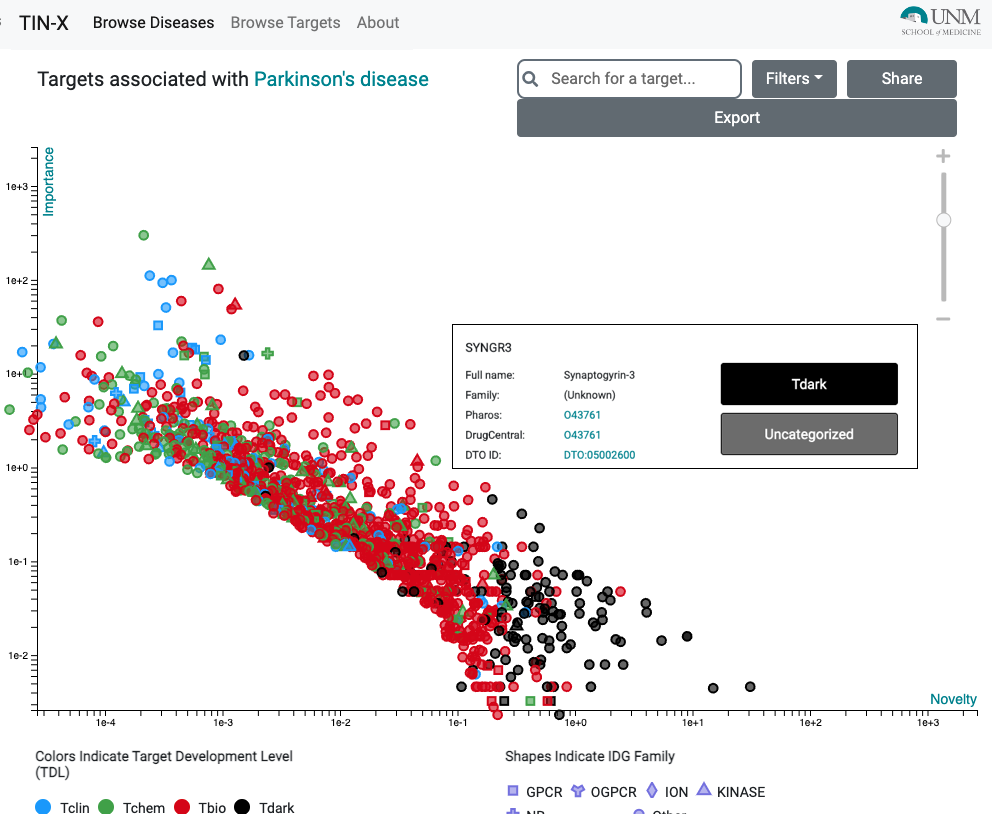
\includegraphics[width=\linewidth]{figures/tinx/TINX_SYNRG3_rev3.png}
    \caption{Screenshot of TIN-X.}
    \label{fig:tinx_01}
\end{figure}

\begin{figure}
    \centering
    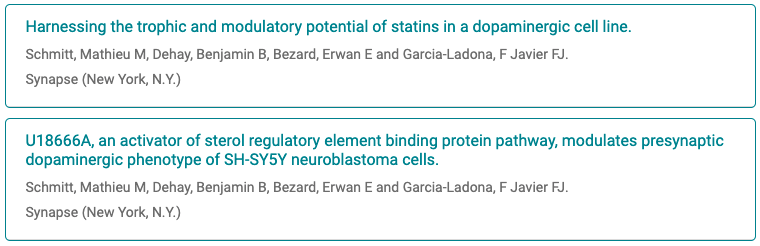
\includegraphics[width=\linewidth]{figures/tinx/TINX_SYNRG3articles_rev2.png}
    \caption{TIN-X articles for gene-disease association}
    \label{fig:tinx_02}
\end{figure}

\subsection{Conclusions}

TIN-X provides an intuitive visualization, ranking, and prioritization platform for scientists interested in potentially novel drug targets, and exploring the relationship between diseases, disease categories, proteins and protein classes, using literature mining.  As with all current text mining, TIN-X cannot replace expert human readers and curators, yet, it is increasingly clear that automated bibliometry is essential given the volume of literature to be processed. The proposed bibliometric variables of merit, Importance and Novelty, plus the non-dominated rank, provide an efficient and intuitive approach for rapid evaluation of the evidence for prioritizing disease-gene associations for illuminating the druggable genome. 

\subsection{Researcher contributions}

TIN-X was originally developed by Cristian Bologa, implemented by Daniel Cannon, and supervised by Tudor Oprea. Subsequent improvements have involved a team effort in which JY has provided a major effort (\href{http://purl.org/spar/scoro/major-effort}{scoro:major-effort}), including:

\begin{itemize}[topsep=0pt,itemsep=0pt,partopsep=0pt,parsep=0pt]
    \item Co-authorship of paper.
    \item Project management for version 2 redesign.
    \item Support, outreach, documentation (see version 2 \href{https://zenodo.org/record/5038628}{poster}).
    \item Application science via KGAP project.
\end{itemize}
